\clearpage
\chapter{\textbf{Foundations}}\label{grundlagen}
%\addtocontents{toc}{\vspace{0.8cm}}
\section{Definitions}
\subsection{IoT and IIoT}
The term Internet of Things was first coined by \cite{ashtonThatInternetThings} when explaining the idea of combining RFID with the internet in an executive meeting. He explains that on the "normal" internet, most of the content is created by human beings. In contrast to this in the Internet of Things the data is generated by things and often describes things. But his emphasizes lays more on the description of things. For example to track and count them. The information to do so would come from sensors and RFID, he says.
Of course in these days more of the information on the internet is generated by bots and AI. But other than that the distinction still holds true. 
\\The Internet Society \cite{roseInternetThingsOverview} further explains that in the Internet of Things, machines are communicating with each other and are addressable via an own IP address. This standardizes the way in which devices communicate. They also mention that "Today, the Internet of Things has become a popular term for describing scenarios in which  Internet connectivity and computing capability extend to a variety of objects, devices, sensors, and everyday  items."
\\The Industrial Internet of Things is just the description of a domain where the IoT is used. In this case in manufacturing. \cite{WhatIoTInternet}
\section{State of the Art}\label{unterkapitel}
\subsection{Industrial IoT Architectures and Patterns}
Due to the requirement that the solution be developed utilizing IoT technologies and is set within a production context, a review of Industrial IoT (IIoT) architectures and patterns was conducted. The Industrial Internet Reference Architecture (IIRA) \cite{youngIndustrialInternetReference2022} serves as a comprehensive framework, offering valuable insights into various architectural models and design patterns relevant to this domain. This reference architecture describes the following patterns: IoT Component Capability Pattern, Three-Tier Architecture Pattern, Gateway-Mediated Edge Connectivity and Management architecture pattern, Digital Twin Core as a Middleware Architecture Pattern, Layered Databus Architecture Pattern, System-of-Systems Orchestrator Architecture Pattern. Of these patterns only the first two are applicable within the scope of this work. Therefore the other ones will only be described on the surface.
\paragraph{Architecture Patterns}
IoT architecture patterns define the structure and operation of various IoT systems, detailing their implementation and highlighting their unique characteristics.
\subparagraph{IoT Component Capability Model Pattern}
A single component and its associated capabilities are described, with the possibility that a component may comprise multiple sub-components. Consequently, the entire system can also be regarded as a component. The specific meanings of the capabilities are illustrated in the accompanying figure.
\begin{figure}[H]
	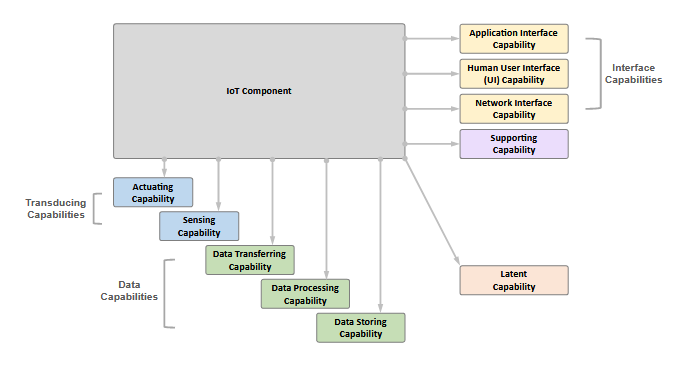
\includegraphics[width=\linewidth]{pic/IIRA-model-component-pattern.png}
	\caption{Component Capability Pattern. \\ (Young et al., 2022, S. 40)}
	\label{fig:Model-Component-Pattern}
\end{figure}
\subparagraph{Three-Tier Architecture Pattern}
The system comprises the Edge, Platform, and Enterprise Tiers, as well as connecting networks. The Edge Tier contains sensors and gateways that collect data. These are connected by the Proximity Network. Data preprocessing may already be happening there.
\\The Platform Tier is responsible for most data processing and storage via databases. It is connected to the Edge Tier via the Access Network.
\\The Enterprise Tier provides domain-specific applications and interfaces for end users. These are built upon the processed data from the platform tier. It also issues controls to lower tiers. This tier is connected to the Access Network via the Service Network.
The three tiers can also be further divided into different domains. That makes sense for bigger systems. But for a simple system as the one described in this work it is not necessary and therefore these domains will not be explained here.
\begin{figure}[H]
	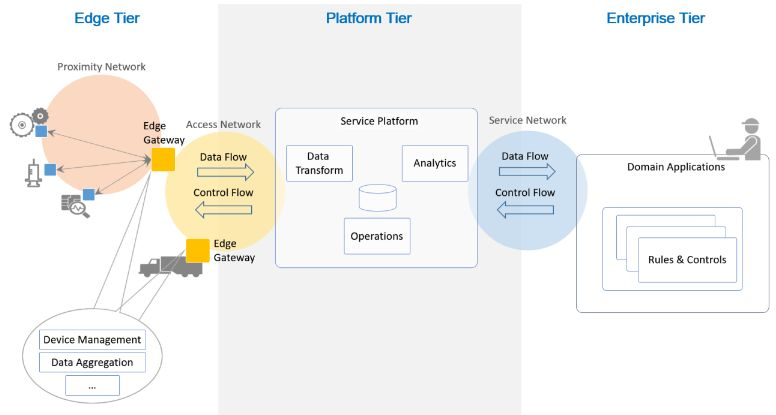
\includegraphics[width=\linewidth]{pic/three-tier-architecture.jpg}
	\caption{Three Tier Architecture \\ (Young et al., 2022, S. 44)}
	\label{fig:Three-Tier-Architecture}
\end{figure}
\subsection{Performance measurement in production environments}

\subsection{IoT-Plattforms}
The IoT is known for producing large amounts of data and for the potentials to grow these amounts even more. Therefore a scalable software infrastructure that is needed. That is where IoT-Plattforms come into play \cite{turkiEvaluatingOpenSource2024}. The authors also mention that IoT-Platforms help accelerating the solution development "[...] by providing foundational capabilities, avoiding the need to implement low-level infrastructure."
\\\cite{asemaniUnderstandingIoTPlatforms2019} further highlight the different capabilities that are typical for IoT-Platforms.
\paragraph{Connectivity and Device Management}
Through various communication protocols the platforms connect with the devices, enabling them to communicate with each other, manage device status and configurations, handle software updates and provide mechanisms for error reporting.
\paragraph{Data Storage, Management, Analysis, Visualization}
Through connections to databases they store large volumes of data often in the cloud or locally. Also further data processing and analytics through various methods as well as visualizations through dashboards are possible.
\paragraph{Development and Deployment Tools}
By providing APIs and SDKs the developers are enabled to further create custom applications.
\paragraph{Auditing and Payments}
The Platforms help to have an overview over the data or compute usage and the resulting costs.
\paragraph{Service Management}
By giving an oversight over parameters like resource consumption, data requirements and access, the user can monitor vertical as well as platform internal services. The platforms also enable the communication between services or combination of basic services to create new ones.
\paragraph{Integration}
Platforms can be integrated with each other, other data sources and the cloud. 
\paragraph{Fog/Edge Computing}
IoT-Platforms often support distributed data processing and storage. This can lead to less traffic due to processing close to the data source. Faster transmission would be enabled therefore and reinforced due to  shorter communication distances.
\\\\The researchers go on to reveal that while commercial platforms carry all of the mentioned capabilities, open source platforms are often focused on specific capabilities. Thus in implementation sometimes need to be combined to deliver a holistic IoT-Platform. 
\subsection{Differences between Relational and Timeseries Databases}
In the paper written by \cite{turkogluComparisonTimeSeries2024} it is analyzed how relational databases and time series databases compare regarding speed and storage efficiency when used in Grafana.
First they point out the use case for relational databases is for single time data points, which can be related to other data points over various tables. Therefore enabling complex queries involving joins, aggregations and multiple tables. They make sure the data is accurate and stays consistent.
Time series data bases on the other hand are made for data points with a timestamp and large volumes of data. This makes them ideal for IoT applications and real time data analytics. They are optimized to enable high speed read and write operations as well as efficient data storage.
The differences in query return time are already there with small amounts of data, but when scaling up the amount they become clearly visible as can be seen in the figure below.
\begin{figure}[H]
	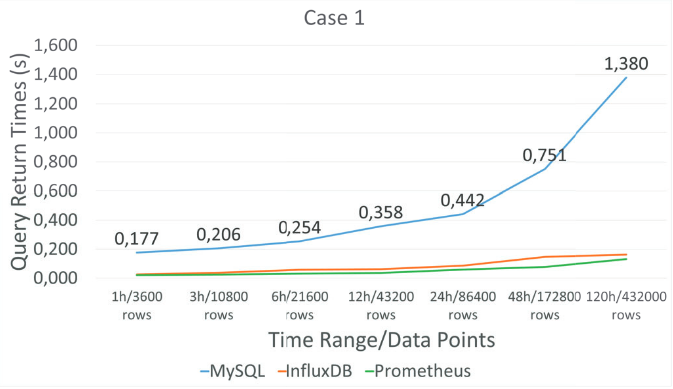
\includegraphics[width=\linewidth]{pic/query-performance-db.png}
	\caption{Query Performance Relational vs. Time Series DB \\ (Turkoglu et. al, 2024, S. 2)}
	\label{fig:query-performance-db}
\end{figure}
This is only one of three test cases but they all give a similar picture that shows the superiority of time series databases regarding query return times.

\subsection{Dashboarding}
\addtocontents{toc}{\vspace{0.8cm}}


